%%%%%%%%%%%%%%%%%%%%%%%%%%  ltexpprt_doublecolumn.tex  %%%%%%%%%%%%%%%%%%%%%%%%%%%%%%%%
%
% This is ltexpprt_twocolumn.tex, an example file for use with the SIAM LaTeX2E
% Preprint Series macros. It is designed to provide two-column output.
% Please take the time to read the following comments, as they document
% how to use these macros. This file can be composed and printed out for
% use as sample output.

% Any comments or questions regarding these macros should be directed to:
%
%                 Donna Witzleben
%                 SIAM
%                 3600 University City Science Center
%                 Philadelphia, PA 19104-2688
%                 USA
%                 Telephone: (215) 382-9800
%                 Fax: (215) 386-7999
%                 e-mail: witzleben@siam.org


% This file is to be used as an example for style only. It should not be read
% for content.

%%%%%%%%%%%%%%% PLEASE NOTE THE FOLLOWING STYLE RESTRICTIONS %%%%%%%%%%%%%%%

%%  1. There are no new tags.  Existing LaTeX tags have been formatted to match
%%     the Preprint series style.
%%
%%  2. Do not change the margins or page size!  Do not change from the default
%%     text font!
%%
%%  3. You must use \cite in the text to mark your reference citations and
%%     \bibitem in the listing of references at the end of your chapter. See
%%     the examples in the following file. If you are using BibTeX, please
%%     supply the bst file with the manuscript file.
%%
%%  4. This macro is set up for two levels of headings (\section and
%%     \subsection). The macro will automatically number the headings for you.
%%
%%  5. No running heads are to be used for this volume.
%%
%%  6. Theorems, Lemmas, Definitions, aligns, etc. are to be double numbered,
%%     indicating the section and the occurrence of that element
%%     within that section. (For example, the first theorem in the second
%%     section would be numbered 2.1. The macro will
%%     automatically do the numbering for you.
%%
%%  7. Figures and Tables must be single-numbered.
%%     Use existing LaTeX tags for these elements.
%%     Numbering will be done automatically.
%%
%%  8. Page numbering is no longer included in this macro.
%%     Pagination will be set by the program committee.
%%
%%
%%%%%%%%%%%%%%%%%%%%%%%%%%%%%%%%%%%%%%%%%%%%%%%%%%%%%%%%%%%%%%%%%%%%%%%%%%%%%%%

%%%%%%%%%%%%%%%%%%%%%% IMR 2025 SUBMISSION INSTRUCTIONS %%%%%%%%%%%%%%%%%%%%%%%
%%  1. Full papers are limited to 12 pages in length (US letter size),
%%     excluding references, and including figures, tables, and appendices. The
%%     paper must be submitted in PDF format.
%%  2. Do not include author names or affiliations in the initial submission.
%%     The review process is double-blind so avoid using terminology that might
%%     reveal your identity.
%%  3. Authors are welcome to submit supplementary material (e.g., code,
%%     datasets, animations, etc.) to the actual paper or research note.
%%     The paper or note must be complete even without the supplementary
%%     material. Note that the supplementary material must
%%     maintain the anonymity of the submission.
%%  4. OpenConf only keeps the last uploaded file so if you have supplementary
%%     material, zip it with the paper and upload that.
%%
%%     Please review https://www.internationalmeshingroundtable.com/imr32/call-for-papers/
%%     carefully to make sure your submission meets all the requirements.

\newcommand\anon[2]{{#2}} %known

\documentclass[twoside,leqno,twocolumn]{article}

\usepackage[letterpaper]{geometry}

\usepackage{ltexpprt}
% defines environments algorithm, theorem, proof
% defines newtheorems: lemma, fact, corollary, Axiom, cond (Condition), property, proposition, Conjecture, Definition, Lemma, Remark, Example, Method, Exercise

\usepackage{hyperref}

% https://www.siam.org/Portals/0/Macros/Online/docsiamonline.pdf
% SIAM journals currently encourage the use of \cref{myfig} and \cref{mysection} instead of e.g. Fig.~\ref{myfig}, \S 1.2 (for section 1.2)
% use \Cref{myref} to capitalize the first letter at the start of sentences
% Note: direct \ref references and other examples of poor style have been modified by Scott A. Mitchell for the IMR Template
\usepackage{amsmath}
\usepackage{cleveref}

%% pseudocode:
%% ltexpprt defines "algorithm" so don't \usepackage{algorithm} to overwrite it. SIAM wants it the way it is, inline and numbered like a theorem or definition, not floating figure-like.
%% Use one of the following four options
%   \usepackage[algo2e]{algorithm2e}   % algo2e parameter avoids name clash with "algorithm" from ltexpprt
%.   \usepackage{algorithmic}
%    \usepackage{algorithmicx} % with algpseudocode
\usepackage{algpseudocode} % with algorithmicx, or by itself

\newtheorem{condition}{Condition}

\usepackage{physics}
\usepackage{fancyvrb}

% Plex operations
\usepackage{bbm}
\def\cone{\mathbbm{cone}}
\def\supp{\mathbbm{supp}}
\def\ornt{\mathbbm{ornt}}
\def\cl{\mathbbm{cl}}
\def\st{\mathbbm{st}}
\def\child{\mathbbm{child}}
\def\parent{\mathbbm{parent}}

% TikZ
\usepackage{tikz}
\usepackage{pgflibraryshapes}
\usetikzlibrary{decorations.text}
\usetikzlibrary{decorations.pathreplacing}
\usetikzlibrary{backgrounds}
\usetikzlibrary{calc}
\usetikzlibrary{arrows}
\usetikzlibrary{snakes}
\usetikzlibrary{positioning}
%%\input{figures/tikzColors}
\definecolor{cffffff}{RGB}{255,255,255}
\definecolor{cff00c0}{RGB}{255,0,192}
\definecolor{c0f00ff}{RGB}{15,0,255}
\definecolor{c00ff20}{RGB}{0,255,32}
\definecolor{cfffd00}{RGB}{255,253,0}
\definecolor{c00e0ff}{RGB}{0,224,255}
\usepackage{pgfplots}
\usepackage{pgfplotstable}

\usepackage{color}
\definecolor{deepblue}{rgb}{0,0,0.5}
\definecolor{deepred}{rgb}{0.6,0,0}
\definecolor{deepgreen}{rgb}{0,0.5,0}
\DeclareFixedFont{\ttb}{T1}{cmtt}{bx}{n}{10} % for bold
\DeclareFixedFont{\ttm}{T1}{cmtt}{m}{n}{10}  % for normal
\DeclareFixedFont{\sttb}{T1}{cmtt}{bx}{n}{8} % for bold
\DeclareFixedFont{\sttm}{T1}{cmtt}{m}{n}{8}  % for normal
\usepackage{listings}
% C style for highlighting
\newcommand\cstyle{\lstset{
language=C,
basicstyle=\sttm,
otherkeywords={MPI_Comm,TS,SNES,KSP,PC,DM,Mat,Vec,VecScatter,IS,PetscSF,PetscSection,PetscObject,PetscInt,PetscScalar,PetscReal,PetscBool,InsertMode,PetscErrorCode}, % Add keywords here
keywordstyle=\sttb\color{deepblue},
emph={PETSC_COMM_WORLD,PETSC_NULL,SNES_NGMRES_RESTART_PERIODIC},          % Custom highlighting
emphstyle=\sttb\color{deepred},    % Custom highlighting style
commentstyle=\sttm\color{brown},
stringstyle=\sttm\color{deepgreen},
frame=tb,                         % Any extra options here
showstringspaces=false,           %
columns=fullflexible              % Necessary for proper cut/paste
}}

\newcommand\cinlinestyle{\lstset{
language=C,
basicstyle=\ttm,
otherkeywords={MPI_Comm,TS,SNES,KSP,PC,DM,Mat,Vec,VecScatter,IS,PetscSF,PetscSection,PetscObject,PetscInt,PetscScalar,PetscReal,PetscBool,InsertMode,PetscErrorCode}, % Add keywords here
keywordstyle=\ttb\color{deepblue},
emph={PETSC_COMM_WORLD,NULL,SNES_NGMRES_RESTART_PERIODIC},          % Custom highlighting
emphstyle=\ttb\color{deepred},    % Custom highlighting style
commentstyle=\ttm\color{brown},
stringstyle=\ttm\color{deepgreen},
frame=tb,                         % Any extra options here
showstringspaces=false,           %
columns=fullflexible              % Necessary for proper cut/paste
}}

% C environment
\lstnewenvironment{cprog}[1][]
{
\cstyle
\lstset{#1}
}
{}

% C for inline
\newcommand\cinline[1]{{\cinlinestyle\lstinline!#1!}}

\begin{document}

%
\newcommand\relatedversion{}
\renewcommand\relatedversion{\thanks{The full version of the paper can be accessed at \anon{\protect\url{redacted-url}}{\protect\url{https://arxiv.org/abs/1902.09310}}}} % Replace URL with link to full paper or comment out this line

\title{\Large Solvers for Cohesive Cell Formulations of Crustal Dynamics}
\anon{
    \author{Submission ID XYZ}  % replace with actual submission id. Keep things anonymous during the double-blind review.
}
{ % Actual author names go below
    \author{Brad Aagaard\thanks{United States Geological Survey} and Matthew G. Knepley\thanks{University at Buffalo} and Charles Williams\thanks{GNS Science}}
}

\date{}

\maketitle

% Copyright Statement
% When submitting your final paper to a SIAM proceedings, it is requested that you include
% the appropriate copyright in the footer of the paper.  The copyright added should be
% consistent with the copyright selected on the copyright form submitted with the paper.
% Please note that "20XX" should be changed to the year of the meeting.

% Default Copyright Statement
% \fancyfoot[R]{\scriptsize{Copyright \textcopyright\ 2025 by SIAM\\
% Unauthorized reproduction of this article is prohibited}}

% Depending on which copyright you agree to when you sign the copyright form, the copyright
% can be changed to one of the following after commenting out the default copyright statement
% above.

\fancyfoot[R]{\scriptsize{Copyright \textcopyright\ 2024\\
Copyright for this paper is retained by authors}}

%\fancyfoot[R]{\scriptsize{Copyright \textcopyright\ 20XX\\
%Copyright retained by principal author's organization}}

%\pagenumbering{arabic}
%\setcounter{page}{1}%Leave this line commented out.

\begin{abstract} \small\baselineskip=9pt Solvers for faults are hard, but we did it.
\end{abstract}


\section{Introduction}

\section{Methodology}

The two solvers presented below make use of the same basic pieces: a separation of the various physicsal fields, a multilevel decomposition, basic iterative methods, and direct solvers. The methods differ in their nested structure, and the scale at which each piece is applied. These choices can be crucial for efficient performance on different architectures and in different rheological regimes.

\subsection{Global Block Solver}

Recall that the equations for a prescribed-slip fault embedded in an elastic medium can be represented linear algebraically as
\begin{align}
  \mqty( E & C \\ C^T & 0) \mqty(u \\ \lambda) = \mqty(f \\ d)
\end{align}
where $E$ is the elastic operator, $C$ describes the slip constraints, $u$ is the displacement field, $\lambda$ the total fault stress, $f$ the elastic body forces, and $d$ the slip distribution. We can globally apply a Schur complement scheme to this matrix using the PETSc FieldSplit preconditioner~\cite{petsc-user-ref,bkmms2012}. Using the full factorization, our preconditioner has the form
\begin{align}
  \mqty( I & -\hat E^{-1} C \\ 0 & I) \mqty(\hat E^{-1} & 0 \\ 0 & \hat S^{-1}) \mqty(I & 0 \\ -C^T \hat E^{-1} & I)
\end{align}
where the Schur Complement $S$ is defined by
\begin{align}
  S = -C^T \hat E^{-1} C
\end{align}
and we have used $\hat A^{-1}$ to indicate an approximate solve for the operator $A$.

The elastic operator can be efficiently inverted using multigrid. Algebraic multigrid (AMG) works well, both ML and GAMG in PETSc, but has some setup penalty. If the mesh is uniformly refined, we can use geometric multigrid for the refinement levels, and then use AMG for the coarse solve. The Schur Complement solve requires a preconditioner for $S$, but it is represented implicitly. The \texttt{selfp} option in PETSc uses the diagonal of $E$ to approximate $S$ for a preconditioning matrix. In our experiments, the convergence of this choice degrades with increasing fault size.

\subsection{Global Multigrid}

We can instead invert the relation between multigrid and block solvers, using multigrid as the overarching solver and block algorithms for the smoothers. The most important consideration is to accurately capture coupling across the fault interface. Pointwise smoothers fail completely in this respect.

We construct the fine grid smoother by first reordering the unknowns so that dofs duplicated by the introduced faults are adjacent. Since the mesh ordering is generally good for banding, the reordering transformation is a greedy algorithm on top of the original ordering. Next we combine unknowns coupled by fault cohesive cells into blocks, which is stored by the PETSc matrix object by marking the start of each block. This blocking is then used by the Variable Point-Block Jacobi (VPBJACOBI) preconditioner to extract and invert these fault blocks. This smoother can be selected for the AMG fine grid, and easily compared with standard choices. In fact, the entire solver can be dynamically assembled at runtime from command line options.

Consider the following mesh with two cohesive cells comprising one fault,
% make -f ./gmakefile test search="dm_impls_plex_tests-ex69_tri_2" EXTRA_OPTIONS="-dm_view :${PWD}/tri_t1.tex:ascii_latex -dm_plex_view_numbers 0 -dm_plex_transform_cohesive_width 0.1"
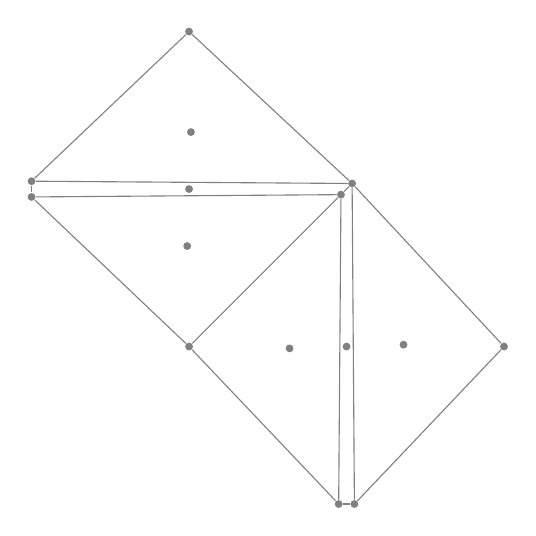
\begin{tikzpicture}[scale = 1.,font=\fontsize{8}{8}\selectfont]
\path (-2.,0.) node(6_0) [fill,inner sep=1pt,shape=circle,color=gray] {};
\path (2.,0.) node(7_0) [fill,inner sep=1pt,shape=circle,color=gray] {};
\path (-2.,4.) node(8_0) [fill,inner sep=1pt,shape=circle,color=gray] {};
\path (0.0707107,2.07071) node(9_0) [fill,inner sep=1pt,shape=circle,color=gray] {};
\path (-0.0707107,1.92929) node(10_0) [fill,inner sep=1pt,shape=circle,color=gray] {};
\path (0.1,-2.) node(11_0) [fill,inner sep=1pt,shape=circle,color=gray] {};
\path (-0.1,-2.) node(12_0) [fill,inner sep=1pt,shape=circle,color=gray] {};
\path (-4.,2.1) node(13_0) [fill,inner sep=1pt,shape=circle,color=gray] {};
\path (-4.,1.9) node(14_0) [fill,inner sep=1pt,shape=circle,color=gray] {};
\draw[color=gray] (6_0) -- (12_0);
\draw[color=gray] (11_0) -- (9_0);
\draw[color=gray] (12_0) -- (10_0);
\draw[color=gray] (9_0) -- (13_0);
\draw[color=gray] (10_0) -- (14_0);
\draw[color=gray] (10_0) -- (6_0);
\draw[color=gray] (14_0) -- (6_0);
\draw[color=gray] (11_0) -- (7_0);
\draw[color=gray] (7_0) -- (9_0);
\draw[color=gray] (9_0) -- (8_0);
\draw[color=gray] (8_0) -- (13_0);
\draw[color=gray] (9_0) -- (10_0);
\draw[color=gray] (11_0) -- (12_0);
\draw[color=gray] (13_0) -- (14_0);
\path (-0.72357,-0.0235702) node(0_0) [fill,inner sep=1pt,shape=circle,color=gray] {};
\path (0.72357,0.0235702) node(1_0) [fill,inner sep=1pt,shape=circle,color=gray] {};
\path (-1.97643,2.72357) node(2_0) [fill,inner sep=1pt,shape=circle,color=gray] {};
\path (-2.02357,1.27643) node(3_0) [fill,inner sep=1pt,shape=circle,color=gray] {};
\path (0.,-5.55112e-17) node(4_0) [fill,inner sep=1pt,shape=circle,color=gray] {};
\path (-2.,2.) node(5_0) [fill,inner sep=1pt,shape=circle,color=gray] {};
\end{tikzpicture}
where we have introduced a fault gap purely to show explicitly the cohesive cells, which in the simulation have zero volume. In~\cref{fig:sparsityC}, we display the sparsity pattern of our operator highlighting only the $C$ and $C^T$ matrices. The red and blue entries indicate the two sides of the fault, which are distinguished by positive and negative terms. The top panel is the sparsity in the original mesh ordering, whereas the bottom has grouped unknowns coupled by cohesive cells into two fault blocks, followed by the usual elastic blocks of size two. We can see the blocking for this mesh in output from PETSc:
\begin{verbatim}
Mat Object: Jacobian 1 MPI process
  type: seqaij
  rows=24, cols=24, bs=2 variable blocks set
  total: nonzeros=320, allocated nonzeros=320
  total number of mallocs used during MatSetValues calls=0
    IS Object: Block Sizes 1 MPI process
      type: general
    Number of indices in set 5
    0 12
    1 6
    2 2
    3 2
    4 2
\end{verbatim}

\begin{figure}
\centering
% make -f ./gmakefile test search="dm_impls_plex_tests-ex5_tri_t1_0" EXTRA_OPTIONS="-local_jacobian_view draw -draw_pause -1 -geometry 0,0,1000,1000"
\includegraphics[width=0.48\textwidth]{figures/TwoFaultSystem.png}
% make -f ./gmakefile test search="dm_impls_plex_tests-ex5_tri_t1_0_perm" EXTRA_OPTIONS="-local_jacobian_view draw -draw_pause -1 -geometry 0,0,1000,1000"
\includegraphics[width=0.48\textwidth]{figures/TwoFaultSystemPerm.png}
\caption{In the top panel, we show the sparsity of our operator highlighting the $C$ and $C^T$ blocks. On the bottom, we show the system permuted for the VPBJACOBI preconditioner.\label{fig:sparsityC}}
\end{figure}

This solver is particularly well-suited to GPUs, as the VPBJACOBI preconditioner has been optimized for this architecture by the libCEED team~\cite{brownbarrabeamsghaffariknepleymosesshakeristengelthompsonzhang2022}

\section{Results}

\section{Conclusion}

\bibliographystyle{siam}
\bibliography{references}

\end{document}
